\subsection{Puntas de osciloscopio}
Una punta de osciloscopio es un dispositivo utilizado para conectar un osciloscopio a un circuito eléctrico que se desea medir. Consta de las siguientes partes:
\begin{itemize}
    \item Conector de entrada: Este es el extremo de la punta que se conecta al osciloscopio generalmente es un conector BNC.
    \item Atenuador: Las puntas de osciloscopio tienen un atenuador incorporado que permite al usuario seleccionar entre diferentes relaciones de atenuación, como 1X, 10X. Esto es útil para adaptar la punta a diferentes niveles de voltaje de la señal que se está midiendo.
    \item Punta de medición: Es la parte de la punta que se conecta al circuito que se está midiendo.
    \item Compensador: El ajuste de compensación se utiliza para corregir la capacitancia inherente de la punta. Esto ayuda a mantener la integridad de la señal y a garantizar mediciones precisas, especialmente en frecuencias bajas.
\end{itemize}

\begin{figure}[H]
    \centering
        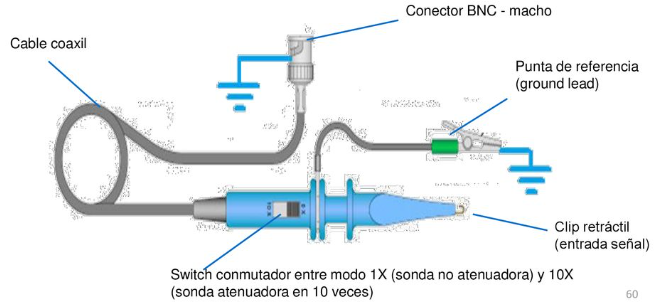
\includegraphics[width=0.9\textwidth]{Imagenes/puntaOsc.PNG}
    \caption{Punta de prueba de oscilocopio y sus partes}
\label{fig:puntaOsc}
\end{figure}

\vspace{0.5cm}
\subsection{Control del osciloscopio}

Un osciloscopio es un instrumento de medición electrónico utilizado para visualizar y analizar señales eléctricas en función del tiempo. Es una herramienta esencial en el campo de la electrónica. Generalmente un osciloscopio esta compuesto por un panel de control que incluye ajustes de posición $x-y$, ajustes de trigger-disaparo y de escala $x_t-y_V$, selectores de acoplamiento (CH1, CH2, etc.) y ajustes generales de brillo y contraste de la pantalla. Además de un pantalla y un panel de entradas que incluye 3 entradas BNC, 2 asociadas al canal 1 y 2, y el tercero para ajustar el nivel de trigger a través de un dispositivo externo (EXT-TR) y una salida asociada a una señal cuadrada estándar utilizado para la calibración del las puntas del osciloscopio.
Ahora se listaran algunos de los elementos más importantes:
    
\subsubsection{Controles verticales}
    
La configuración del eje vertical nos permite variar el modo y la escala en la cual se va a mostrar las señales entrantes en los canales CH1 y CH2.
    
    \begin{itemize}
            \item Modo de acoplamiento: El acoplamiento del eje vertical permite mostrar distintos componentes de la señal entrante al osciloscopio. Existen 3 modos de acoplamiento:
            \begin{itemize}
                \item Acoplamiento DC: En este modo, la señal se muestra tal como es, incluidas las componentes de corriente continua.
                \item Acoplamiento AC: En este modo, mediante un capacitor, se bloquea cualquier componente de corriente continua de la señal, lo que significa que solo se muestran las componentes de corriente alterna. El capacitor que hace posible esto, puede influir en el circuito y deformar la imagen de la señal.
                \item Acoplamiento GND:
                En este modo se desconecta  la señal de entrada proveyendo una señal constante de $0V$ útil para ajustar la posición de la señal sobe el eje vertical.
        \end{itemize}
        
        \item Dial de $Volts$ por división (V/div): El selector esta compuesto de dos diales que nos permiten modificar la escala del eje vertical y un factor de atenuación, que generalmente varía entre una sensibilidad de $1:1$ hasta $100:1$.
        \item Selectora de modo vertical: La selectora de modo vertical nos permite seleccionar que es lo que se muestra en la pantalla. Existen 5 modos de los cuales 2 corresponden a las entradas \textit{CH1} y \textit{CH2}, otra para el modo $x-y$, el cual asocia las entradas a los ejes horizontal y vertical respectivamente, el modo \textit{DUAL}, que permite ver ambas señales en simultaneo (canal 1 y 2) y el modo \textit{ADD} el cual suma las señales de las entradas.       
\end{itemize}

\subsection{Controles del eje horizontal}
La configuración del eje horizontal compone todas las modificaciones con respecto a las escalas de tiempo.
\begin{itemize}
    \item Dial de Tiempo por división (t/div): Este dial permite modificar la escala de tiempo mostrada en la pantalla.
    \item Posición Horizontal: Controla la posicion horizontal de las señales visualizadas. 
    \item Modo XY: Muestra un gráfico de la señal de canal 1 en la escala vertical versus la señal del canal 2 en la escala horizontal
    \item Time base \begin{itemize}
        \item Main: Seleccion y ajuste de la base de tiempo principal.
        \item Delayed: Seleccion y ajuste horizontal de la base de tiempo retardada.
        \item Mixed: Seleccion y ajuste horizontal de la base de tiempo principal y retardada para ser visualizadas en un mismo barrido en la pantalla 
    \end{itemize}
\end{itemize}

\subsection{Controles de TRIGGER}
\label{MCtrigger}
El TRIGGER (disparo) en un osciloscopio es una función crucial que permite sincronizar la visualización de la señal en la pantalla con un evento específico de la señal de entrada. Sin el trigger, la forma de onda podría aparecer de manera inestable o desplazada en la pantalla, lo que dificultaría su análisis.
\begin{itemize}
    \item Dial del TRIGGER LEVEL: Este dial determina el punto en la señal de trigger en el cual se realizara el barrido de la señal de entrada. Permitiendo sincronizar el barrido con la señal de entrada.
    \item Selectora TRIGGER SOURCE: Esta selectora permite variar la fuente de señal del disparo. Existen 6 opciones en esta selectora:
    \begin{itemize}
        \item CH1/CH2: Permite cambiar entre las señales de disparo del canal 1 y 2 independientemente del modo vertical. 
        \item ALT: Alterna entre las señales de disparo entre el canal 1 y 2 (comúnmente utilizado en el modo DUAL).
        \item LINE: LINE/linea se refiere a que la señal de disparo es derivada a través de una señal de $50Hz-60Hz$.
        \item EXT: La señal de disparo sera ahora la asociada a la entrada EXT-TR.
    \end{itemize}
    \item Selectora de modo de barrido:
    La selectora nos permite variar entre 4 tipos de modo distintos:
    \begin{itemize}
        \item AUTO: Selecciona el modo de disparo automático. En este modo, el osciloscopio genera barridos en ausencia de un disparo adecuado; automáticamente vuelve a la operación de barrido disparado cuando está presente una señal de disparo adecuada.
        \item NORM: En este modo se genera un barrido cuando se cumple cierta condición en la señal de disparo.
        \item TV-V: Es utilizado para señales de television con sincronizacion verticales.
        \item TV-H: Es mayormente utilizado para señales de television con sincronizacion horizontales.
        \item SINGLE: Algunos osciloscopios digitales posen la opcion de operar en este modo. En este modo, tras pulsar la tecla Run/Stop, el osciloscopio espera para el disparo. Mientras se produce el disparo, el osciloscopio registra una forma de onda y, luego, para.


\item Dial de HOLDOFF-CHOP: El dial de HOLDOFF ajusta el periodo de inactividad entre barridos del disparo. Además este dial puede controlar el perido del el recorte de la función CHOP en el modo vertical DUAL.
    \end{itemize}
\end{itemize}


